%%%%%%%%%%%%%%%%%%%%%%%%%%%%%%%%%%%%%%%%%%%%%%%%%%%%%%%%%%%%%%%%%%%%%%%%%%%%
%% Trim Size: 9.75in x 6.5in
%% Text Area: 8in (include Runningheads) x 5in
%% ws-mpla.tex   :   29-9-2008
%% TeX file to use with ws-mpla.cls written in Latex2E.
%% The content, structure, format and layout of this style file is the
%% property of World Scientific Publishing Co. Pte. Ltd.
%% Copyright 1995, 2002 by World Scientific Publishing Co.
%% All rights are reserved.
%%%%%%%%%%%%%%%%%%%%%%%%%%%%%%%%%%%%%%%%%%%%%%%%%%%%%%%%%%%%%%%%%%%%%%%%%%%%
%%

\documentclass{ws-mpla}
\pdfoutput=1
\usepackage[super]{cite}
\usepackage{graphicx,color,url,hyperref}
\bibliographystyle{ws-mpla}
\hypersetup{colorlinks=true,linkcolor=blue,citecolor=magenta,filecolor=magenta,urlcolor=cyan}
\newcommand{\madanalysis}{{\sc MadAnalysis~5}}

\begin{document}

\markboth{Jongwon Lim, Chih-Ting Lu, Jae-hyeon Park and Jiwon Park}{Implementation of the ATLAS-SUSY-2018-04 analysis in the \madanalysis\ framework}

%%%%%%%%%%%%%%%%%%%%% Publisher's Area please ignore %%%%%%%%%%%%%%
\catchline{}{}{}{}{}
%%%%%%%%%%%%%%%%%%%%%%%%%%%%%%%%%%%%%%%%%%%%%%%%%%%%%%%%%%%%%%%%%%%

\title{IMPLEMENTATION OF THE ATLAS-SUSY-2018-04 ANALYSIS IN THE MADANALYSIS 5 FRAMEWORK}

\author{\footnotesize JONGWON LIM}
\address{
  Department of Physics, Hanyang University, Seoul 04763, Republic of Korea}

\author{\footnotesize CHIH-TING LU}
\address{
  School of Physics, KIAS, Seoul 02455, Republic of Korea}

\author{\footnotesize JAE-HYEON PARK}
\address{
  School of Physics, KIAS, Seoul 02455, Republic of Korea}

\author{\footnotesize JIWON PARK}
\address{
  Department of Physics, Hanyang University, Seoul 04763, Republic of Korea}
\maketitle

\pub{Received (Day Month Year)}{Revised (Day Month Year)}

\begin{abstract}
We present the \madanalysis\ implementation and validation of the ATLAS-SUSY-2018-04 search.
This ATLAS analysis targets direct stau production in events with two hadronic tau leptons, and probes 139 fb$^{-1}$ of LHC proton-proton collisions at a center-of-mass energy of 13 TeV.
The validation of our reimplementation relies on a comparison of our cutflow predictions with the auxiliary material and official results provided by the ATLAS collaboration in the context of two supersymmetry-inspired simplified benchmark models in which the Standard Model is extended by a neutralino and a stau decaying into a tau lepton and a neutralino. {\color{red} Add some quantitative statement about the obtained level of agreement.}
% \keywords{supersymmetry; stau; hadronic tau lepton.}
\end{abstract}

%\ccode{PACS Nos.: include PACS Nos.}

\section{Introduction}

\begin{figure}[t]
  \centerline{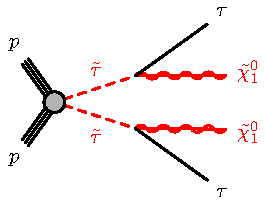
\includegraphics[width=2.0in]{fig_01}}
  \vspace*{8pt}
  \caption{The Feynman diagram for the process $pp\rightarrow\tilde{\tau}\tilde{\tau}\rightarrow\tilde{\chi}^0_1\tilde{\chi}^0_1\tau\tau$.\protect\label{fig:fig_01}}
\end{figure}

In this note, we describe the validation of the implementation, in the \madanalysis\ framework~\cite{Conte:2018vmg,Dumont:2014tja,Conte:2014zja,Conte:2012fm}, of the ATLAS-SUSY-2018-04 search~\cite{Aad:2019byo} for direct stau production in events featuring two hadronic tau leptons and a large amount of missing transverse energy ($E^{miss}_T$).
This analysis focuses on LHC proton-proton collisions at a center-of-mass energy of 13 TeV, and considers an integrated luminosity of $139 {\rm fb}^{-1}$.
The typical supersymmetric signal which this analysis is dedicated to is illustrated by the representative Feynman diagram shown in Fig.~\ref{fig:fig_01}. 

For the validation of our reimplementation, we have focused on a simplified model in which only a few electroweakly-interacting superpartners are relevant.
The lightest neutralino ($\tilde{\chi}^0_1$) is taken as the lightest supersymmetric particle (LSP).
The stau-left ($\tilde{\tau}_L$) and stau-right ($\tilde{\tau}_R$) sleptons are moreover assumed to be mass degenerate and they do not mix. Therefore the gauge eigenstates ($\tilde{\tau}_L$,$\tilde{\tau}_R$) coincide with the mass eigenstates ($\tilde{\tau}_1$,$\tilde{\tau}_2$) in this theoretical framework.
Furthermore, in order to suppress any other decay modes of the tau sleptons, the masses of all charginos and neutralinos are set to 2.5 TeV except for the $\tilde{\chi}^0_1$ neutralino. 
Hence, the single kinematically allowed decay mode of the staus is 
\begin{equation}
\tilde{\tau}\rightarrow\tilde{\chi}^0_1 \tau 
\end{equation}
Finally, all squarks, that do not contribute at leading-order, are decoupled as well.

{\color{red}Add a paragraph detailing the content of the note: in Sec.~X, we present... Sec.~Y is dedicated to... {\it etc.} }

\section{Description of the analysis}

This analysis targets a final state containing two hadronic tau leptons with a certain amount of missing transverse energy. 
The kinematics of the di-$\tau +E^{miss}_T$ system is used to reduce the contributions from Standard Model backgrounds. 
In Sec.~\ref{sec:obj}, we first detail how the objects relevant for the analysis are reconstructed and defined. Then, in Sec.~\ref{sec:selection}, we discuss the sequence of event selections that are applied in the aim of unravelling the signal from the background.

\subsection{Object definitions}\label{sec:obj}

Jets are reconstructed by means of the anti-$k_t$ algorithm~\cite{Cacciari:2008gp} with a radius parameter set to $R=0.4$. This analysis focuses on jets whose transverse momentum $p^j_T$ and pseudorapidity $\eta^j$ fullfill
\begin{equation}
p^j_T > 20 \textrm{ GeV}\quad \textrm{and}\quad |\eta^j| < 2.8.
\end{equation} 
Moreover, the selected jets that are tagged as originating from the fragmentation of a $b$-quark must satisfy the stronger requirements
\begin{equation}
p^b_T > 20 \textrm{ GeV}\quad \textrm{and}\quad |\eta^b| < 2.5.
\end{equation}
In the considered analysis, a $b$-tagging working point with an average efficiency of $77\%$ is used. This working point corresponds to $c$-jet and light-jet rejection rates of $4.9$ and $110$, respectively.

Electron candidates are required to have a transverse momentum $p^e_T$ and pseudorapidity $\eta^e$ obeying
\begin{equation}
p^e_T > 17 \textrm{ GeV}\quad \textrm{and}\quad |\eta^e| < 2.47.
\end{equation}
Furthermore, all electron candidates are required to have both track and calorimeter isolations. The condition of the track isolation is
\begin{equation}
\sum p_{T,\textrm{tracks}}/p^e_T < 0.15\quad \textrm{with}\quad \Delta R=\min(10\textrm{ GeV}/p^e_T,0.2),
\end{equation}
the condition of the calorimeter isolation is
\begin{equation}
\sum E_{T,\textrm{calorimeter}}/p^e_T < 0.2\quad \textrm{with}\quad \Delta R=0.2,
\end{equation}
and for high transverse momentum electron, we use instead of the two above conditions
\begin{equation}
\sum E_{T,\textrm{tracks}} < max(0.015\times p^e_T,3.5\textrm{ GeV})\quad \textrm{with}\quad \Delta R=0.2\quad \textrm{if}\quad p^e_T > 200\textrm{ GeV}.
\end{equation}

Muon candidate definition is similar, although with slightly looser thresholds,
\begin{equation}
p^{\mu}_T > 14 \textrm{ GeV}\quad \textrm{and}\quad |\eta^{\mu}| < 2.7,
\end{equation}
The condition of the track isolation is 
\begin{equation}
\sum p_{T,\textrm{tracks}}/p^{\mu}_T < 0.15\quad \textrm{with}\quad \Delta R=\min(10\textrm{ GeV}/p^{\mu}_T,0.3),
\end{equation}
and the condition of the calorimeter isolation is
\begin{equation}
\sum E_{T,\textrm{tracks}}/p^{\mu}_T < 0.3\quad \textrm{with}\quad \Delta R=0.2.
\end{equation}

In the ATLAS experiment, hadronically decaying tau lepton ($\tau_{had}$) candidates are reconstructed with one or three associated charged pion tracks (prongs).
For 1-prong (3-prong) $\tau$ lepton candidates, the signal efficiencies are $75\%$ and $60\%$ for the \textit{medium} working point respectively.
In the recasting based on \madanalysis\ that we implement in this work, the simulation of the detector response is performed with the {\sc Delphes}~3~\cite{deFavereau:2013fsa} software. We consider a tau-tagging efficiency of $100\%$ with a misidentification probability of $0\%$ at the level of {\sc Delphes}~3, and handle medium and tight tau-tagging efficiencies through event reweighting factors extracted from the official ATLAS cutflow tables. Those factors are evaluated and included at the level of the analysis. Further details are given in Sec.~\ref{sec:selection}.

Baseline tau lepton candidates are required to have 
\begin{equation}
p^{\tau}_T > 50\ (40) \textrm{ GeV}\quad \textrm{and}\quad |\eta^{\tau}| < 2.5
\end{equation}
for the leading (subleading) candidates, and the transition region between the barrel and endcap calorimeters ($ 1.37 < |\eta^{\tau}| < 1.52 $) is excluded.

The object definition ends with some overlap removal conditions. The latter are implemented consistently to the analysis code provided through HEPData\cite{hepdata}.
Tau leptons are removed if they are too close to an electron or a muon, with $\Delta R(\tau,e/\mu) < 0.2$. Electrons are then removed if they are too close to a muon, with $\Delta R(e,\mu) < 0.01$. Next, the jet collection is cleaned from those jets lying at an angular distance $\Delta R(j,e/\mu) < 0.2$ of a muon or an electron, and the electrons and muons that are too close to any of the remaining jets are removed if $\Delta R(e/\mu,j) < 0.4$. Finally, jets are removed if they are too close to one of the tau lepton candidates, with $\Delta R(j,\tau) < 0.4$.


\subsection{Event selection}\label{sec:selection}
{\color{red}The next paragraphs should be clarified. There are so many reweighting factors... I would introduce the section by 2-3 sentences listing the different reweighting factors that will be considered, and the continue with the paragraphs describing all of them.}

After the object definitions introduced in the previous subsection, events with exactly two baseline tau leptons are selected.
All events are required to pass either an \textit{asymmetric di-$\tau$} trigger for the low stau mass region (SR-lowMass) or a combined \textit{di-$\tau +E^{miss}_T$} ($E^{miss}_T > 150$ GeV) trigger for the high stau mass region (SR-highMass). This is coined \textit{trigger and offline cuts} below.
A trigger efficiency of $80\%$ is applied in our recasting, after that we impose that the transverse momenta of the two leading tau candidates are larger than the offline $p_T$ thresholds given in Table~\ref{tab:trig-eff}. {\color{red}Please give information on how the code selects which trigger cuts should be used (2018 or 2015-2017).}
Assuming the tau leptons fired trigger path are selected in offline event selection, trigger level $\tau_{had}$ identification efficiency ($\sim 0.9$) for the offline tau lepton identified with medium identification is applied per selected tau lepton~\cite{ATLAS:2017mpa}.

\begin{table}[t]
  \tbl{Offline $p_T$ thresholds for the leading (subleading) tau lepton candidate, in the case of the \textit{asymmetric di-$\tau$} (second column) and \textit{di-$\tau +E^{miss}_T$} (third column) triggers. This corresponds to a ditau efficiencies of about $80\%$.}
  {\begin{tabular}{@{}c c c@{}} \toprule
  Year & \textit{asymmetric di-$\tau$} & \textit{di-$\tau +E^{miss}_T$} \\
  \colrule
 2015-2017 & 95 (60) GeV & 50 (40) GeV \\
 2018 & 95 (75) GeV & 75 (40) GeV \\ 
  \botrule
  \end{tabular}\label{tab:trig-eff} }
\end{table}

Then events with exactly two \textit{medium} tau lepton candidates with opposite-sign electric charge (OS) are selected. To treat the efficiency of selecting two offline medium tagged taus on top of \textit{di-tau(+$E^{miss}_T$)} trigger, reweighting factor of 0.7 is applied. It is the ratio of cut efficiencies between ATLAS and recasting result without including medium tau identification at \textbf{2 medium $\tau$ (OS) and 3rd medium $\tau$ veto} step.

In the next selection steps, a $b$-jet veto is enforced to reject events originating from top quark processes.
Also, events featuring any additional light leptons (muons or electrons) are rejected.
Finally, selection cuts common to both signal regions also include constraints on the reconstructed invariant mass of the two leading tau lepton system, $m(\tau_1,\tau_2)$. The latter is required to be larger than $120$ GeV, in order to remove events exhibiting a pair of tau leptonrs stemming from low-mass resonances, $Z$ boson, and Higgs boson decays ($Z/H$ veto).

In the SR-lowMass region, a missing energy constraint of 75~GeV $< E^{miss}_T < 150$~GeV is imposed to increase the signal sensitivity. Moreover, the two selected tau leptons are required to be tight tagged.
The selection efficiency $p_{tight}$ associated with two {\it medium} taus passing the \textit{tight} working point requirements is extracted from the official ATLAS cutflow tables. We rely on the ratio of the number of surviving weighted events before applying the tight tau lepton requirement, and after applying it. We use $p_{tight}\simeq 0.70$.

In the SR-highMass region, the tight tagging efficiency is extracted similarly, with the exception that at least one of two tau leptons should pass the tight selection requirements 9and not both of them). We use here $p_{tight} + 2\sqrt{p_{tight}}(1-\sqrt{p_{tight}})\simeq 0.91$.

The \textit{stransverse mass} $m_{T2}$ variable~\cite{Lester:1999tx,Cheng:2008hk} {\color{red}[please add these two references]} is defined as
\begin{equation}
m_{T2} =min_{\mathbf{q}_T}
\left[
max(m_{T,\tau_1}(\mathbf{p}_{T,\tau_1},\mathbf{q}_T),m_{T,\tau_2}(\mathbf{p}_{T,\tau_2},\mathbf{p}^{miss}_T -\mathbf{q}_T))
\right],
\end{equation}   
where $\mathbf{p}_{T,\tau_1}$ and $\mathbf{p}_{T,\tau_2}$ are the transverse momenta of the two tau lepton candidates. The transverse momentum vector of one of the invisible particle, $\mathbf{q}_T$, is choosen to minimize the larger of the two transverse mass $m_{T,\tau_1}$ and $m_{T,\tau_2}$. The transverse mass $m_T$ is defined by
\begin{equation}
m_{T}(\mathbf{p}_T,\mathbf{q}_T) = \sqrt{2(p_T q_T -\mathbf{p}_T\cdot\mathbf{q}_T)}.
\end{equation} 
In \madanalysis, the $m_{T2}$ calculation can be done automatically through the function {\tt PHYSICS->Transverse->MT2(vec1,vec2,ETmiss,Minvisible)}. In this expression, {\tt vec1} and {\tt vec2} stand for the two visible momenta, {\tt ETmiss} for the miissing transverse momentum and {\tt Minvisible} for a test mass that should map the expected mass of the invisible state.

A lower bound on the $m_{T2}$ variable of 70~GeV is imposed, in order to reduce the contamination from $t\overline{t}$ and $WW$ events.
Finally, the two tau lepton candidates are required to be well separated in the transverse plane, by $\Delta R(\tau_1,\tau_2) < 3.2$ and $|\Delta\phi (\tau_1,\tau_2)| > 0.8$ to further suppress the contributions of the Standard Model backgrounds.


\section{Validation}

\subsection{Event generation}

In order to validate our analysis, we rely on the MSSM implementation~\cite{Duhr:2011se} available in the {\sc Feynrules}~\cite{Alloul:2013bka} model database and shipped with thew {\sc MadGraph5\_aMC@NLO} event generator~\cite{Alwall:2014hca} as a UFO library~\cite{Degrande:2011ua}.{\color{red}Add the generic UFO reference.}

We consider two benchmark points with masses $m(\tilde{\tau},\tilde{\chi}^0_1)=(120,1)$ GeV and $(280,1)$ GeV to illustrate the validation of our reimplementation, as those correspond two scenarios for which official ATLAS cutflows and differential distributions are provided.
The stau mixing matrix is additionally set to a unity matrix, so that the stau mass-eigenstates correspond to the right-handed and left-handed stau flavor-eigenstates.

We make use of MADGRAPH5 aMC@NLO version 2.6.7~\cite{Alwall:2014hca} for hard-scattering event generation for each of the two stau eigenstates, in which we convolute leading-order matrix elements with the NNPDF23LO~\cite{Ball:2013hta} set of parton distribution function. {\color{red} Fix the NNPDF reference.} Our signal matrix elements include the potential emission of up to two additional partons, and the different contributions are merged according to the MLM scheme~\cite{Mangano:2006rw,Alwall:2008qv}. We use a merging scale defined through the hard-scattering level parameter of {\sc MadGraph5\_aMC2NLO} {\tt xqcut} $= m_{\tilde{\tau}}/4$.

The {\sc Pythia} package version 8.244~\cite{Sjostrand:2014zea} with the so-called $A14$ tune\cite{} has been used for the simulation of parton showering and hadronization. {\color{red}Fix the pythia reference and add an A14 reference}. The simulation of the detector response has been performed by using {\sc Delphes}~3.4.2~\cite{deFavereau:2013fsa}, that relies on {\sc FastJet}~\cite{Cacciari:2011ma} for object reconstruction.

We have tuned the ATLAS detector parameterization in {\sc Delphes}~3 appropriately, according to the needs of the analysis.
For example, loosened isolation criteria are applied so that isolation could be implemented fully at the analysis level.
Moreover, the radius parameter and minimum transverse momentum used for jet reconstruction are reduced to 0.4 and 15~GeV respectivey, and we have updated the $b$-tagging and tau-tagging performance.
Finally, the {\tt UniqueObjectFinder} module has been disabled as object overlap removal has been implemented at the level of the analysis.



\subsection{Comparison with the official results}
In Tables~\ref{tab:120GeV} and~\ref{tab:280GeV}, we compare predictions obtained with our implementation to the official results provided in the form of auxiliary tables by the ATLAS collaboration, for the two considered benchmark points with masses $m(\tilde{\tau},\tilde{\chi}^0_1)=(120,1)$ and $(280,1)$ GeV respectively.
For each cut, we have calculated the related efficiency
\begin{equation}
\epsilon_i =\frac{n_i}{n_{i-1}}
\end{equation}
where $ n_i $ and $ n_{i-1} $ correspond to the number of events after and before the considered cut respectively.
%
On the other hand, we have also evaluated the differences between the \madanalysis\ ($\epsilon_i ({\rm MA5})$) and ATLAS ($\epsilon_i ({\rm ATLAS})$) cut efficiencies through the quantity
\begin{equation}
\delta_i = \frac{\epsilon_i ({\rm MA5})-\epsilon_i ({\rm ATLAS})}{\epsilon_i ({\rm ATLAS})}.
\end{equation}
{\color{red}Need to mention that MA5 is weighted to have same yield of ATLAS at Baseline cut?}


\begin{table}[t]
\renewcommand{\arraystretch}{1.3}
  \tbl{Cut-flow associated with a simplified model benchmark scenario defined by $ m(\tilde{\tau},\tilde{\chi}^0_1) = (120,1) $~GeV and for the $ pp\to \tilde{\tau}\tilde{\tau} $ production process. We compare ATLAS official results and \madanalysis\ predictions through the expected number of events after each cut and the corresponding efficiencies, and indicate their difference $\delta$.}
  {\begin{tabular}{@{}c c c c c c@{}} \toprule
\multicolumn{6}{c}{ \textbf{$ \tilde{\tau}\tilde{\tau} $ production with $ m(\tilde{\tau},\tilde{\chi}^0_1) = (120,1) $ GeV} }\\
 & ATLAS ($N_{weighted}$) & $\epsilon_i$($\%$) & MA5 ($N_{weighted}$) & $\epsilon_i$($\%$) & diff.($\%$) \\
\hline
Baseline cut                                    &  1686.80 &     - &  1686.80 &     - &      - \\ \hline
%
\multicolumn{5}{c}{ \textbf{SR-low Mass} }\\\hline
Trigger and offline cuts                        &   390.46 & 23.15 &   410.01 & 24.31 &   5.01 \\
2 medium $\tau$ (OS) and 3rd medium $\tau$ veto &   256.01 & 65.57 &   269.37 & 65.70 &   0.20 \\
$b$-jet veto                                    &   250.59 & 97.88 &   263.66 & 97.88 &  -0.00 \\
Light lepton veto                               &   250.12 & 99.81 &   263.66 &   100 &   0.19 \\
$Z/H$-veto                                      &   248.93 & 99.52 &   262.14 & 99.42 &  -0.10 \\
$ 75 < E^{miss}_T < 150 $ GeV                   &    85.70 & 34.43 &    89.90 & 34.30 &  -0.38 \\
2 tight $\tau$                                  &    60.19 & 70.23 &    62.93 & 70.00 &  -0.33 \\
$ |\Delta\phi(\tau,\tau)| > 0.8 $               &    60.14 & 99.92 &    62.75 & 99.72 &  -0.20 \\
$ |\Delta R(\tau,\tau)| < 3.2 $                 &    54.73 & 91.00 &    57.10 & 90.99 &  -0.01 \\
$ m_{T2} > 70 $ GeV                             &     9.78 & 17.87 &    14.65 & 25.66 &  43.58 \\
All                                             &        - &  0.58 &        - &  0.87 &  49.80 \\
%
\multicolumn{5}{c}{ \textbf{SR-high Mass} }\\\hline
Trigger and offline cuts                        &   101.23 &  6.00 &    96.35 &  5.71 &  -4.82 \\
2 medium $\tau$ (OS) and 3rd medium $\tau$ veto &    67.04 & 66.23 &    63.23 & 65.62 &  -0.91 \\
$b$-jet veto                                    &    63.98 & 95.44 &    60.37 & 95.47 &   0.04 \\
Light lepton veto                               &    63.87 & 99.83 &    60.36 & 99.99 &   0.16 \\
$Z/H$-veto                                      &    58.33 & 91.33 &    55.70 & 92.28 &   1.04 \\
$ \geq 1 $ tight $\tau$                         &    57.29 & 98.22 &    50.69 & 91.00 &  -7.35 \\
$ |\Delta\phi(\tau,\tau)| > 0.8 $               &    56.71 & 98.99 &    49.99 & 98.63 &  -0.36 \\
$ |\Delta R(\tau,\tau)| < 3.2 $                 &    51.74 & 91.24 &    45.41 & 90.84 &  -0.43 \\
$ m_{T2} > 70 $ GeV                             &     7.18 & 13.88 &     8.24 & 18.14 &  30.75 \\
All                                             &        - &  0.43 &        - &  0.49 &  14.76 \\ \botrule
\end{tabular}
\label{tab:120GeV} }
\end{table}

\begin{table}[t]
\renewcommand{\arraystretch}{1.3}
  \tbl{Same as in Table~\ref{tab:120GeV} but for a scenario with supersymmetric masses $ m(\tilde{\tau},\tilde{\chi}^0_1) = (280,1) $ GeV.}
  {\begin{tabular}{@{}c c c c c c@{}} \toprule
\multicolumn{6}{c}{ \textbf{$ \tilde{\tau}\tilde{\tau} $ production with $ m(\tilde{\tau},\tilde{\chi}^0_1) = (280,1) $ GeV} }\\
 & ATLAS ($N_{weighted}$) & $\epsilon_i$($\%$) & MA5 ($N_{weighted}$) & $\epsilon_i$($\%$) & diff.($\%$) \\
\hline
Baseline cut                                    &   184.36 &     - &   184.36 &     - &      - \\ \hline
%
\multicolumn{5}{c}{ \textbf{SR-low Mass} }\\\hline
Trigger and offline cuts                        &    73.74 & 40.00 &    69.97 & 37.95 &  -5.12 \\
2 medium $\tau$ (OS) and 3rd medium $\tau$ veto &    47.86 & 64.90 &    46.23 & 66.08 &   1.81 \\
$b$-jet veto                                    &    46.63 & 97.43 &    44.94 & 97.20 &  -0.24 \\
Light lepton veto                               &    46.49 & 99.70 &    44.94 & 99.99 &   0.30 \\
$Z/H$-veto                                      &    44.84 & 96.45 &    43.83 & 97.54 &   1.13 \\
$ 75 < E^{miss}_T < 150 $ GeV                   &    17.48 & 38.98 &    16.26 & 37.10 &  -4.83 \\
2 tight $\tau$                                  &    12.04 & 68.88 &    11.38 & 70.00 &   1.63 \\
$ |\Delta\phi(\tau,\tau)| > 0.8 $               &    12.04 &   100 &    11.33 & 99.55 &  -0.45 \\
$ |\Delta R(\tau,\tau)| < 3.2 $                 &    11.08 & 92.03 &    10.35 & 91.32 &  -0.77 \\
$ m_{T2} > 70 $ GeV                             &     6.08 & 54.87 &     5.64 & 54.50 &  -0.68 \\
All                                             &        - &  3.30 &        - &  3.06 &  -7.24 \\
%
\multicolumn{5}{c}{ \textbf{SR-high Mass} }\\\hline
Trigger and offline cuts                        &    47.64 & 25.84 &    42.10 & 22.83 & -11.64 \\
2 medium $\tau$ (OS) and 3rd medium $\tau$ veto &    30.72 & 64.48 &    27.80 & 66.03 &   2.40 \\
$b$-jet veto                                    &    29.34 & 95.51 &    26.83 & 96.52 &   1.06 \\
Light lepton veto                               &    29.27 & 99.76 &    26.83 & 99.99 &   0.23 \\
$Z/H$-veto                                      &    24.88 & 85.00 &    24.01 & 89.50 &   5.30 \\
$ \geq 1 $ tight $\tau$                         &    24.21 & 97.31 &    21.85 & 91.00 &  -6.48 \\
$ |\Delta\phi(\tau,\tau)| > 0.8 $               &    23.29 & 96.20 &    21.19 & 96.96 &   0.79 \\
$ |\Delta R(\tau,\tau)| < 3.2 $                 &    21.95 & 94.25 &    19.68 & 92.91 &  -1.42 \\
$ m_{T2} > 70 $ GeV                             &    14.35 & 65.38 &    13.37 & 67.91 &   3.88 \\
All                                             &        - &  7.78 &        - &  7.25 &  -6.84 \\ \botrule
\end{tabular}
\label{tab:280GeV} }
\end{table} 

We observe that for both scenarios, a good agreement is obtained at each step of the cutflow, with the exception of the last cut on the $M_{T2}$ variable. For the $m(\tilde{\tau},\tilde{\chi}^0_1)=(120,1) $~GeV scenario, we hence obtain a disagreement of 30\%--40\% for both signal regions. In constrast, for the $m(\tilde{\tau},\tilde{\chi}^0_1)=(280,1)$~GeV scenario does not feature any strong issue at all, the two cutflow agreeing at the level of a few percent.

By lack of additional publicly available experimental information, we have not been able to investigate this issue at a very deep level. We have nevertheless compared $M_{T2}$ distributions as predicted by \madanalysis\ after all cuts, to those released by the ATLAS collaboration\cite{hepdata}. We have considered the two signal regions and both scenarios. Our results are shown in Fig.~\ref{fig:mt2}.

We observe that the global shape of the distribution is generally well reproduced, although the curves exhibit large differences that explain our findings at the level of the cutflow tables. However, one must note that the differences concern cases where a not so large number of (unweighted) events survive. Large Monte Carlo uncertainties of 10\%--20\% of percent are thus expected, both for our predictions and the ATLAS results.

On different lines, the number of signal events after all cuts are in the same ballpark, so that the potential impact on limit setting is mild. For this reason, the good agreement for one of the two benchmarks and the global reproduction of the $M_{T2}$ shapes for both scenarios, we consider this reimplementation as validated.
{\color{red}Please check that you are happy with everything (re)written above,}

\begin{figure}[t]
  \centerline{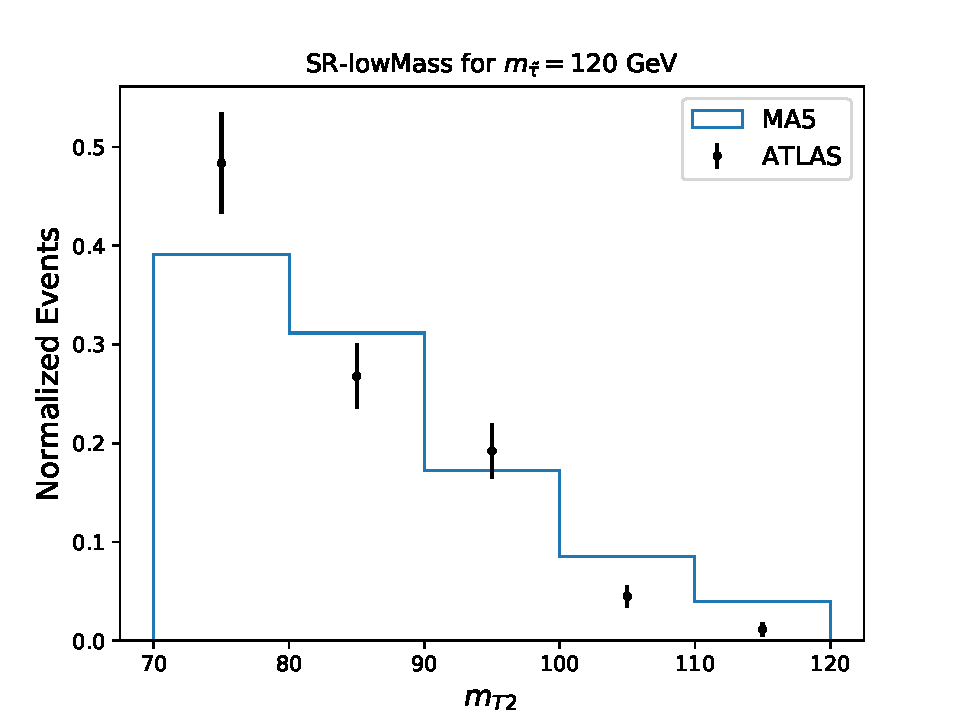
\includegraphics[width=2.0in]{m120_SRlow}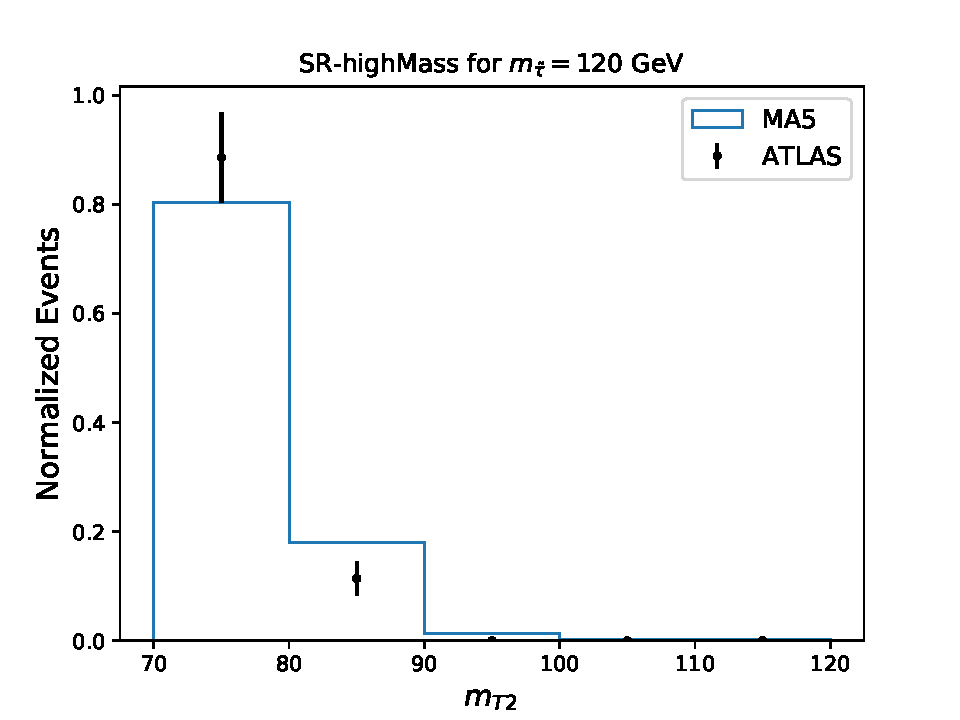
\includegraphics[width=2.0in]{m120_SRhigh}}
  \vspace*{8pt}
  \centerline{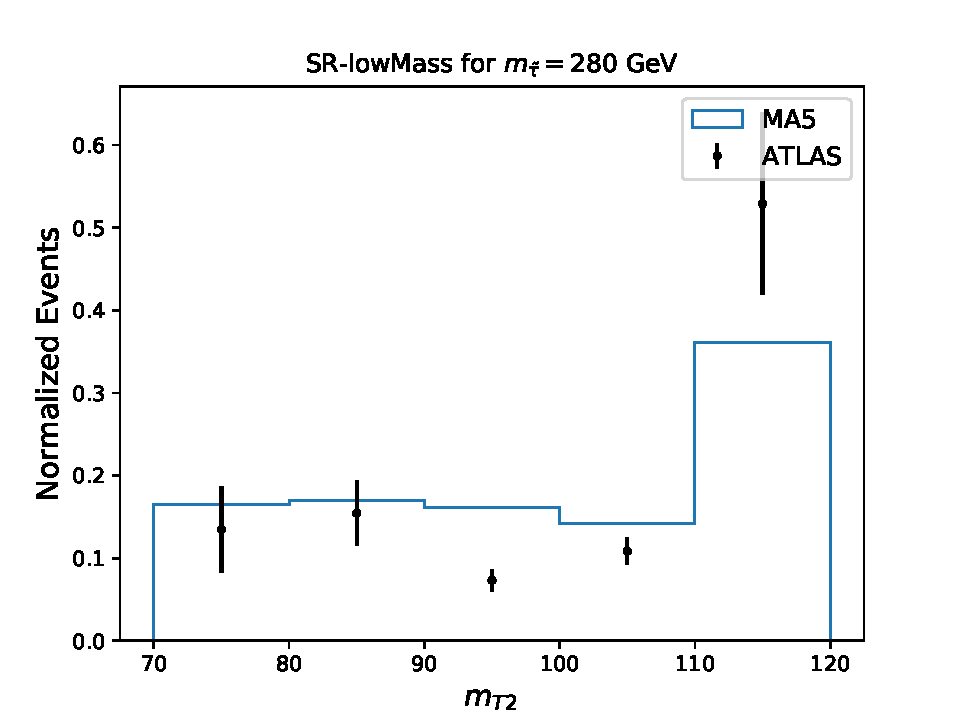
\includegraphics[width=2.0in]{m280_SRlow}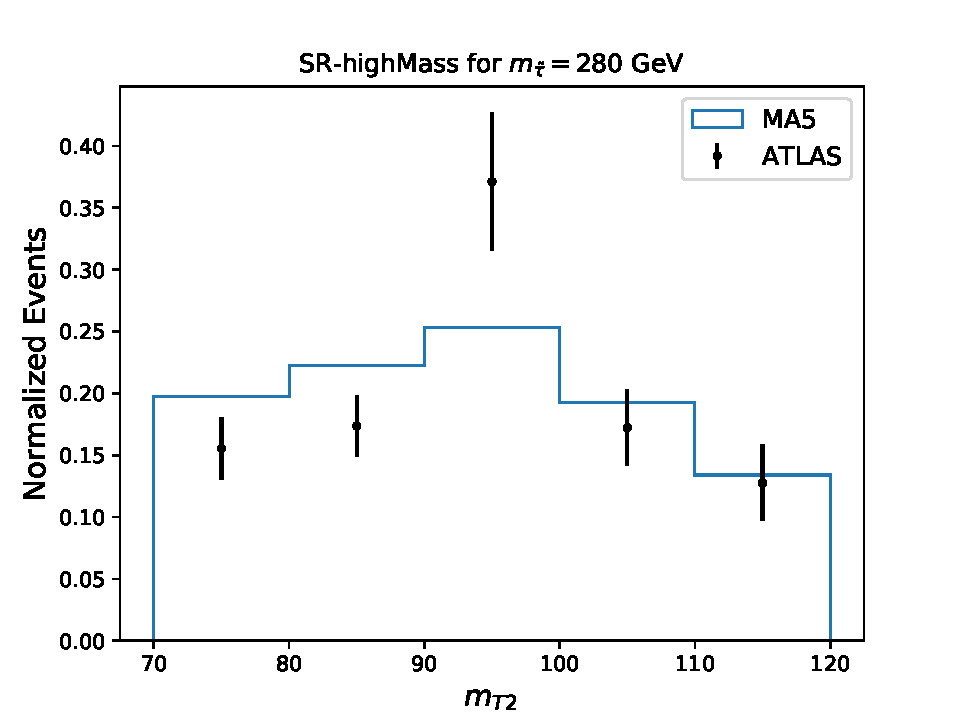
\includegraphics[width=2.0in]{m280_SRhigh}}
  \caption{The $m_{T2}$ distributions after all cuts, for the SR-low Mass (left) and SR-high Mass (right) signal regions, and for the $m(\tilde{\tau},\tilde{\chi}^0_1)=(120,1)$~GeV (top panel) and $m(\tilde{\tau},\tilde{\chi}^0_1)=(280,1)$~GeV (bottom panel) scenarios.\protect\label{fig:mt2}}
\end{figure}


\section{Conclusions}

In this note, we detail our implementation of the ATLAS-SUSY-2018-04 search in the \madanalysis\ framework. Our analysis has been validated in the context of a supersymmetry-inspired simplified benchmark model in which the Standard Model is extended by a neutralino and a stau. Both stau chiralities are considered, as the stau is considered to decay into a tau lepton and a neutralino. Our validation relies on two different benchmark points in the parameter space.

By comparing our predictions for different cutflows for the two benchmarks with the official ones provided by the ATLAS collaboration in Ref.~[\refcite{Aad:2019byo}], we have found an agreement at each step of the analysis, except for the last cut on the stranverse mass variable $m_{T2}$ cut for the light stau scenario. While the shape of the distribution is correctly reproduced, large difference leads to a quite different cut efficiency. Due to the lack of more information, we have however not been able to investigate the issue more precisely.

As we got an agreement at the level of a few percent for the heavy stau scenario, and that the discrepancies for the light stau scenarios are connected with large Monte Carlo uncertainties (and are thus less significant), we have considered our reimplementation as validated.

%\section*{Acknowledgments}
%Dedications and funding information may be included here.
% add acknowledgments of basic kias grant (CT) and NRF grant (JP)

\begin{thebibliography}{99}
\bibitem{Conte:2018vmg}
  E.~Conte and B.~Fuks,
  Int.\ J.\ Mod.\ Phys.\ A {\bf 33} (2018) no.28,  1830027
  [arXiv:1808.00480 [hep-ph]].

\bibitem{Dumont:2014tja}
  B.~Dumont {\it et al.},
  Eur.\ Phys.\ J.\ C {\bf 75} (2015) no.2,  56
  [arXiv:1407.3278 [hep-ph]].

\bibitem{Conte:2014zja}
  E.~Conte, B.~Dumont, B.~Fuks and C.~Wymant,
  Eur.\ Phys.\ J.\ C {\bf 74} (2014) no.10,  3103
  [arXiv:1405.3982 [hep-ph]].

\bibitem{Conte:2012fm}
  E.~Conte, B.~Fuks and G.~Serret,
  Comput.\ Phys.\ Commun.\  {\bf 184} (2013) 222
  [arXiv:1206.1599 [hep-ph]].

%\cite{Aad:2019byo}
\bibitem{Aad:2019byo} 
  G.~Aad {\it et al.} [ATLAS Collaboration],
  %``Search for direct stau production in events with two hadronic $\tau$-leptons in $\sqrt{s} = 13$ TeV $pp$ collisions with the ATLAS detector,''
  Phys.\ Rev.\ D {\bf 101}, no. 3, 032009 (2020)
  doi:10.1103/PhysRevD.101.032009
  [arXiv:1911.06660 [hep-ex]].
  %%CITATION = doi:10.1103/PhysRevD.101.032009;%%
  %7 citations counted in INSPIRE as of 27 Mar 2020

%\cite{Aad:2019byo}
\bibitem{hepdata}
G.~Aad \textit{et al.} [ATLAS],
%``Search for direct stau production in events with two hadronic $\tau$-leptons in $\sqrt{s} = 13$ TeV $pp$ collisions with the ATLAS detector,''
doi:10.17182/hepdata.92006
%https://doi.org/10.17182/hepdata.92006

%\cite{Cacciari:2008gp}
\bibitem{Cacciari:2008gp} 
  M.~Cacciari, G.~P.~Salam and G.~Soyez,
  %``The anti-$k_t$ jet clustering algorithm,''
  JHEP {\bf 0804}, 063 (2008)
  doi:10.1088/1126-6708/2008/04/063
  [arXiv:0802.1189 [hep-ph]].
  %%CITATION = doi:10.1088/1126-6708/2008/04/063;%%
  %6790 citations counted in INSPIRE as of 27 Mar 2020

%\cite{Duhr:2011se}
\bibitem{Duhr:2011se} 
  C.~Duhr and B.~Fuks,
  %``A superspace module for the FeynRules package,''
  Comput.\ Phys.\ Commun.\  {\bf 182}, 2404 (2011)
  doi:10.1016/j.cpc.2011.06.009
  [arXiv:1102.4191 [hep-ph]].
  %%CITATION = doi:10.1016/j.cpc.2011.06.009;%%
  %69 citations counted in INSPIRE as of 27 Mar 2020
  
%\cite{Alloul:2013bka}
\bibitem{Alloul:2013bka} 
  A.~Alloul, N.~D.~Christensen, C.~Degrande, C.~Duhr and B.~Fuks,
  %``FeynRules  2.0 - A complete toolbox for tree-level phenomenology,''
  Comput.\ Phys.\ Commun.\  {\bf 185}, 2250 (2014)
  doi:10.1016/j.cpc.2014.04.012
  [arXiv:1310.1921 [hep-ph]].
  %%CITATION = doi:10.1016/j.cpc.2014.04.012;%%
  %1327 citations counted in INSPIRE as of 27 Mar 2020

%\cite{Alwall:2014hca}
\bibitem{Alwall:2014hca} 
  J.~Alwall {\it et al.},
  %``The automated computation of tree-level and next-to-leading order differential cross sections, and their matching to parton shower simulations,''
  JHEP {\bf 1407}, 079 (2014)
  doi:10.1007/JHEP07(2014)079
  [arXiv:1405.0301 [hep-ph]].
  %%CITATION = doi:10.1007/JHEP07(2014)079;%%
  %4502 citations counted in INSPIRE as of 27 Mar 2020
    
%\cite{Martin:2009iq}
\bibitem{Martin:2009iq} 
  A.~D.~Martin, W.~J.~Stirling, R.~S.~Thorne and G.~Watt,
  %``Parton distributions for the LHC,''
  Eur.\ Phys.\ J.\ C {\bf 63}, 189 (2009)
  doi:10.1140/epjc/s10052-009-1072-5
  [arXiv:0901.0002 [hep-ph]].
  %%CITATION = doi:10.1140/epjc/s10052-009-1072-5;%%
  %4803 citations counted in INSPIRE as of 27 Mar 2020  
  
%\cite{Mangano:2006rw}
\bibitem{Mangano:2006rw} 
  M.~L.~Mangano, M.~Moretti, F.~Piccinini and M.~Treccani,
  %``Matching matrix elements and shower evolution for top-quark production in hadronic collisions,''
  JHEP {\bf 0701}, 013 (2007)
  doi:10.1088/1126-6708/2007/01/013
  [hep-ph/0611129].
  %%CITATION = doi:10.1088/1126-6708/2007/01/013;%%
  %695 citations counted in INSPIRE as of 27 Mar 2020

%\cite{Alwall:2008qv}
\bibitem{Alwall:2008qv} 
  J.~Alwall, S.~de Visscher and F.~Maltoni,
  %``QCD radiation in the production of heavy colored particles at the LHC,''
  JHEP {\bf 0902}, 017 (2009)
  doi:10.1088/1126-6708/2009/02/017
  [arXiv:0810.5350 [hep-ph]].
  %%CITATION = doi:10.1088/1126-6708/2009/02/017;%%
  %210 citations counted in INSPIRE as of 27 Mar 2020  

%\cite{Sjostrand:2007gs}
\bibitem{Sjostrand:2007gs} 
  T.~Sjostrand, S.~Mrenna and P.~Z.~Skands,
  %``A Brief Introduction to PYTHIA 8.1,''
  Comput.\ Phys.\ Commun.\  {\bf 178}, 852 (2008)
  doi:10.1016/j.cpc.2008.01.036
  [arXiv:0710.3820 [hep-ph]].
  %%CITATION = doi:10.1016/j.cpc.2008.01.036;%%
  %5077 citations counted in INSPIRE as of 27 Mar 2020

%\cite{deFavereau:2013fsa}
\bibitem{deFavereau:2013fsa} 
  J.~de Favereau {\it et al.} [DELPHES 3 Collaboration],
  %``DELPHES 3, A modular framework for fast simulation of a generic collider experiment,''
  JHEP {\bf 1402}, 057 (2014)
  doi:10.1007/JHEP02(2014)057
  [arXiv:1307.6346 [hep-ex]].
  %%CITATION = doi:10.1007/JHEP02(2014)057;%%
  %1518 citations counted in INSPIRE as of 27 Mar 2020

%\cite{Cacciari:2011ma}
\bibitem{Cacciari:2011ma} 
  M.~Cacciari, G.~P.~Salam and G.~Soyez,
  %``FastJet User Manual,''
  Eur.\ Phys.\ J.\ C {\bf 72}, 1896 (2012)
  doi:10.1140/epjc/s10052-012-1896-2
  [arXiv:1111.6097 [hep-ph]].
  %%CITATION = doi:10.1140/epjc/s10052-012-1896-2;%%
  %3362 citations counted in INSPIRE as of 27 Mar 2020

%\cite{ATLAS:2017mpa}
\bibitem{ATLAS:2017mpa}
  ATLAS Collaboration,
  %``Measurement of the tau lepton reconstruction and identification performance in the ATLAS experiment using $pp$ collisions at $\sqrt{s}=13~{\rm TeV}$,''
  ATLAS-CONF-2017-029.
  %113 citations counted in INSPIRE as of 11 Nov 2020
\end{thebibliography}
\end{document}
